\documentclass{beamer}
\usepackage[ngerman]{babel}
\usepackage{booktabs}
\usepackage{tabulary}
\usepackage{siunitx}

\usetheme{imise}
\author{Konrad Höffner}
\date{2017-05-16, Institutskolloquium}
\title{Tools der SNIK Ontologie}
%\institute{IMISE Institutskolloquium}
\subtitle{\url{https://github.com/KonradHoeffner/latex/releases/download/colloquium/colloquium.pdf}}
\newcommand{\todo}[1]{TODO: #1}
\newcommand{\imageslide}[2]
{
%\usebackgroundtemplate{\includegraphics[height=1.05\textheight]{#1}}
%\usebackgroundtemplate{\includegraphics[width=1.07\textwidth]{#1}}
\begin{frame}{#1}
\centering\includegraphics[width=1\textwidth,height=0.8\textheight,keepaspectratio]{#2}
\end{frame}
%\usebackgroundtemplate{}
}

\begin{document}
\begin{frame}
\titlepage
\end{frame}

\begin{frame}{SNIK Ontologie}
\begin{itemize}
\item Semantisches Netz des Informationsmanagements im Krankenhaus
\item Fakten aus Lehrbüchern extrahiert
\item Handmodelliertes Metamodell
\item $\approx \num{4000}$ Klassen, 32 Properties, $\approx \num{82000}$ Tripel
\end{itemize}
\end{frame}

\begin{frame}{Einsatz}
\begin{tabular}{ll}
\toprule
\textbf{Ziel}	&\textbf{Zielgruppe}\\
\midrule
Lehre			&Lehrer und Studenten\\ 
Datenintegration	&Krankenhausleitung, CIO\\
Formalisierung		&Domänenexperten, Ontologen\\
\bottomrule
\end{tabular}
\end{frame}

\begin{frame}{RDF Dump in Protégé}
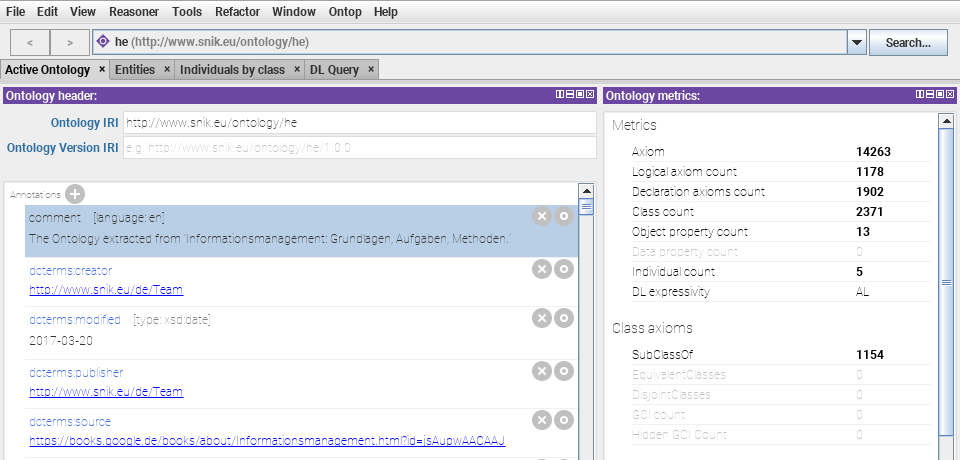
\includegraphics[width=\textwidth]{img/protege.png}
\end{frame}

\begin{frame}{Einsatz}
\begin{tabulary}{\textwidth}{lLL}
\toprule
\textbf{Ziel}		&\textbf{Zielgruppe}		&\textbf{Wünsche}\\
\midrule
Formalisierung		&Domänenexperten, Ontologen	&RDF Dump, Statistiken, Evaluation, Ticketsystem\\
~\\
Lehre			&Lehrer und Studenten		&Visualisierung, RDF-Browser\\
~\\
Datenintegration	&Krankenhausleitung, CIO	&SPARQL-Endpunkt, Dokumentation\\
\bottomrule
\end{tabulary}
\end{frame}

\imageslide{Protégé}{img/protege.png}
\imageslide{Visualisierung I---Cytoscape.js}{img/graph-entitytype.png}
\imageslide{Visualisierung II---Cytoscape.js}{img/graph-erf.png}
\imageslide{SPARQL Endpoint}{img/sparqlresult.png}
\imageslide{RDF Browser---LodLive}{img/browse-cio.png}
\imageslide{Dashboard---Sgvizler}{img/dashboard-medley.png}


% --- alt 
\begin{frame}{Ziele}
\begin{itemize}
\item freie Verfügbarkeit
\item Datensicherung
\item Qualitätskontrolle und -verbesserung
\pause
\item Services für Mensch \& Maschine
\item Effiziente Entwicklung und Qualitätskontrolle
\end{itemize}
\end{frame}

\section{Services}
\begin{frame}{Services für Menschen}
\begin{itemize}
\item Visualisierung: Gesamtüberblick, Beziehungen zwischen den Klassen
\item Browsing: Detailansicht einer Klasse
\item Qualitätskontrolle: Kontrolle zufällige Stichproben
\item Ticketsystem: Melden zufällig entdeckter Fehler 
\item Social Media: Facebook, Twitter, technisches Blog
\end{itemize}
\end{frame}

\begin{frame}
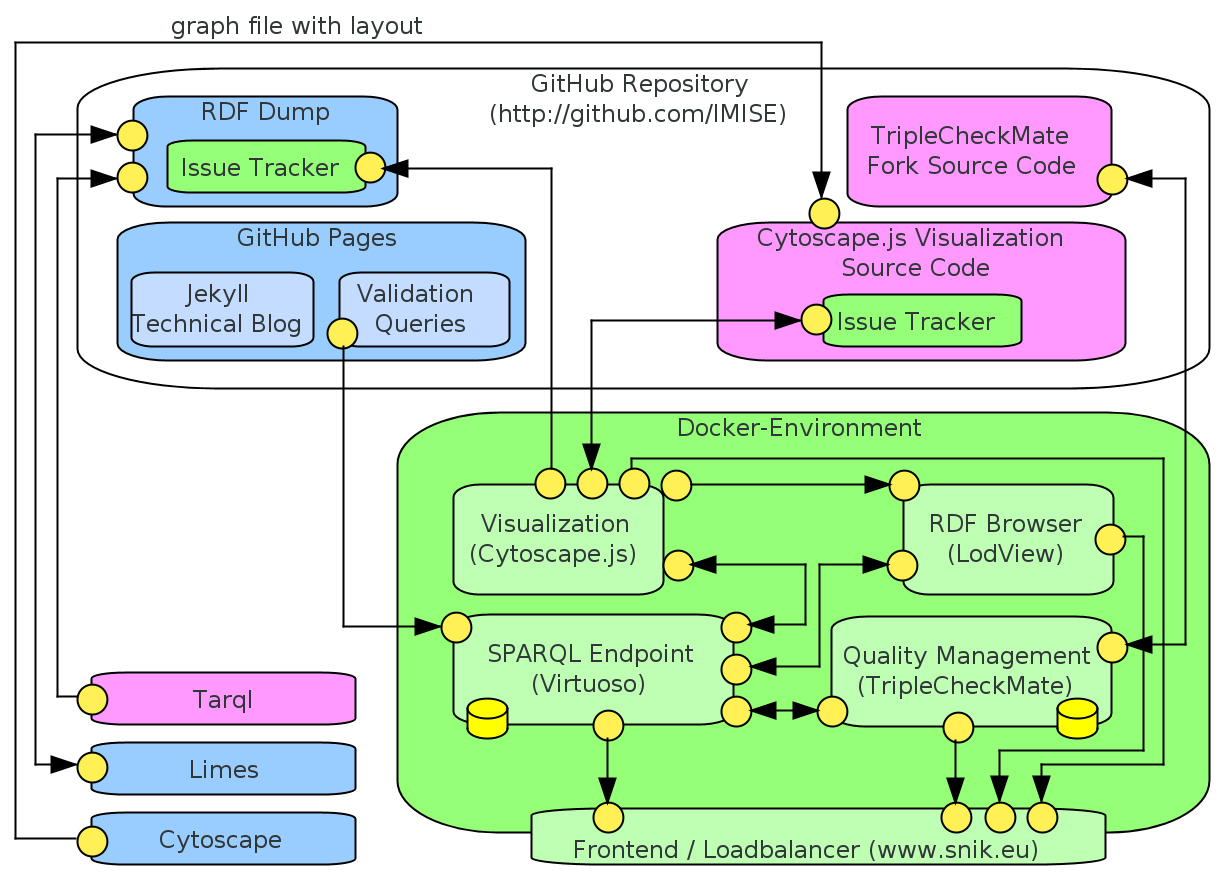
\includegraphics[width=\textwidth]{img/architecture.png}
\end{frame}

\begin{frame}{Services für Maschinen}
\begin{itemize}
\item Serialisiertes RDF: RDF/XML kann von fast allen Tools gelesen werden, z.B. Protégé
\item SPARQL Endpunkt für formale Abfragen, externe Services, z.B. LodLive   
\end{itemize}
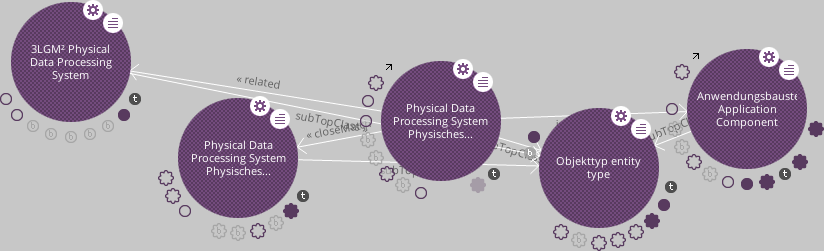
\includegraphics[width=\textwidth]{img/lodlive.png}
\end{frame}


\begin{frame}{Service: Graphvisualisierung}
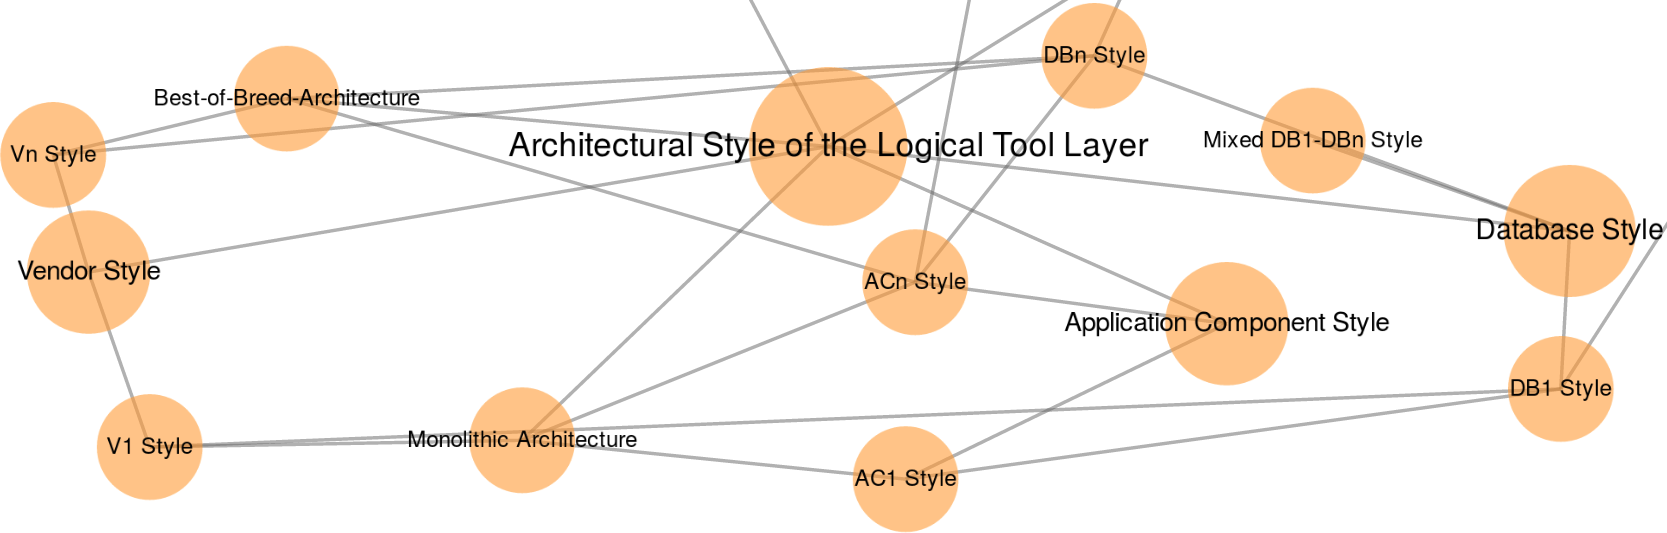
\includegraphics[width=\textwidth]{img/graph.png}
\begin{itemize}
\item \url{http://www.snik.eu/graph}: Öffentliche, stabile Version
\end{itemize}
\end{frame}


\begin{frame}{Ziele I}
\begin{itemize}
\item Konvertieren der Extraktionstabellen zu RDF/OWL Teilontologien 
\item Metaontologie + Teilontologien = konsistente und zusammenhängende SNIK Ontologie 
\end{itemize}
\end{frame}

\begin{frame}{Konvertierung}
\begin{itemize}
\item Ursprünglich: Eigenentwicklung Excel2OWL 
\item Gut an Aufgabe angepasst aber hoher Aufwand für Entwicklung, Wartung und Anpassung, daher Ablösung durch Tarql Konvertierungstool
\item nur noch Konfigurationsdatei (3-4 Seiten) nötig
\item SPARQL-ähnliche Syntax, keine Programmierkenntnisse nötig
\end{itemize}
\end{frame}

\begin{frame}{Interlinking}
\begin{itemize}
\item Verknüpfungen zwischen Klassen verschiedener Teilontologien
\item unterschiedliche Personen extrahieren die Teilontologien 
\item manuelle Interlinks wurden erstellt aber nicht vollständig da hoher Aufwand
\item Ontologien N und M: $|N| \cdot |M|$ potentielle Links
\item LIMES von AKSW um Axel Ngonga
\item Finden von Kandidaten durch Stringähnlichkeit, manuelle Verifizierung und Kategorisierung
\end{itemize}
\end{frame}


\begin{frame}{Effizienz}
\begin{itemize}
\item begrenzte Projektlaufzeit \& Anzahl von Entwicklern aber viele Ziele
\item Einbeziehung von Benutzern bei der Qualitätskontrolle 
\item Verwendung von etablierten Tools und Bibliotheken 
\item Keine Rücksicht auf veraltete Systeme
\item Tools und Beratung durch Arbeitsgruppe AKSW der Uni Leipzig
\item Komponenten als Docker Container durch Sebastian Stäubert 
\end{itemize}
\end{frame}


%\begin{frame}{}
%\end{frame}

\iffalse
\begin{frame}{ownCloud vs Github}
\begin{tabulary}{\textwidth}{lLL}
\toprule
			&ownCloud					&GitHub\\
\midrule
Historie		&willkürlich, unvollständig, nicht garantiert	&vollständig\\
Daten			&alles						&Textdateien, Binärdateien zu Releases\\
Zugriff			&Lesen und Schreiben nur für Mitglieder		&Lesen für alle, Schreiben für Mitglieder, Pull-Requests\\
Backup			&manuell					&GitHub Server + lokale Kopien\\
\bottomrule
\end{tabulary}
\end{frame}

\begin{frame}{ownCloud vs Github}
\begin{tabulary}{\textwidth}{lLL}
\toprule
			&ownCloud					&GitHub\\
\midrule
Bedienung		&synchronisiertes Verzeichnis, Webclient	&Konsole, Client, IDE-Integrationen\\
Mehrbenutzer		&Datenverlust					&halbautomatische Zusammenführung\\
Teilsynchronisation	&möglich					&nicht möglich\\
\bottomrule
\end{tabulary}
\end{frame}
\fi

\begin{frame}
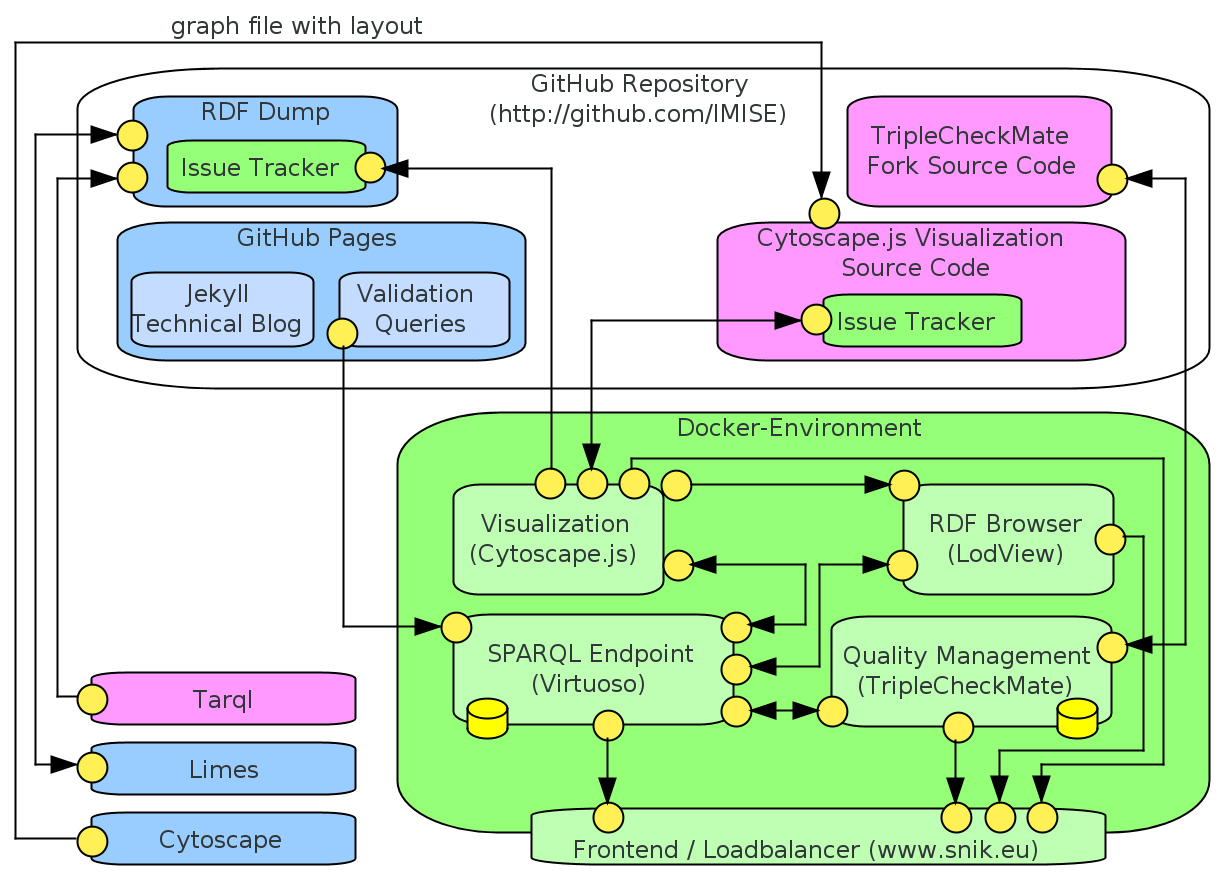
\includegraphics[width=\textwidth]{img/architecture.png}
\end{frame}

\begin{frame}{Ausblick}
\begin{itemize}
\item Weitere Teilontologien 
\item Integration mit elektronischen Lehrbüchern
\item stabilen Zustand erreichen vor Personalengpässen und dann beibehalten
\item Bekanntmachen des Projektes
\item Beiträge durch Community: Instanzdaten, Qualitätskontrolle, Services, Mashups 
\end{itemize}
\end{frame}

\begin{frame}[fragile]{Fragen?}
\begin{itemize}
\item Diese Präsentation \url{https://github.com/KonradHoeffner/latex/releases/download/colloquium/colloquium.pdf}
\vspace{0.5em}%here it works as intended
\item Überblick \url{http://www.snik.eu}
\item Visualisierung \url{http://www.snik.eu/graph}
\item SPARQL Endpunkt \url{http://www.snik.eu/sparql}
\item RDF Browser \url{http://www.snik.eu/ontology}
\item Evaluation \url{http://www.snik.eu/evaluation}
\item Twitter \url{https://twitter.com/snik\_proj}
\item Technisches Blog \url{https://imise.github.io/snik-ontology}
\item GitHub Organisation mit Ticketsystem \url{https://github.com/imise}
\end{itemize}
\end{frame}

\begin{frame}[fragile]{Externe Tools und Bibliotheken}
\begin{itemize}
\item LIMES Interlinker \url{http://aksw.org/Projects/LIMES}
\item Tarql Konvertierungstool \url{https://tarql.github.io/}
\item Cytoscape.js Graphbibliothek \url{http://js.cytoscape.org/}
\item Cytoscape Desktopvisualisierung \url{http://www.cytoscape.org/}
\end{itemize}
\end{frame}
 
\end{document}
